\documentclass{beamer}
\usepackage{graphicx,movie15}


\begin{document}
\begin{frame}[fragile]{Embedding a video with \emph{movie15}}{}
  \begin{block}{}
    \begin{itemize}
      \item Uses \emph{Screen annotations} introduced in PDF 1.5.
      \item Embeds the video data directly inside the generated
            PDF file.
      \item Also generates a \emph{File Attachment annotation},
            allowing easy extraction of the media file from the
            document (in PDF viewers that supports this type of
            annotation).
    \end{itemize}
  \end{block}

  \begin{block}{Example}
    \begin{verbatim}
\includemovie[controls,
  text={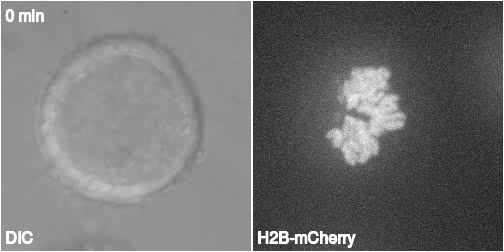
\includegraphics[scale=.3]{testvideo.png}}]{}{}%
  {testvideo.avi}
    \end{verbatim}
  \end{block}
\end{frame}

\begin{frame}{Embedding a video with \emph{movie15}}{}
  \begin{block}{}
    \begin{center}
      \includemovie[controls,
        text={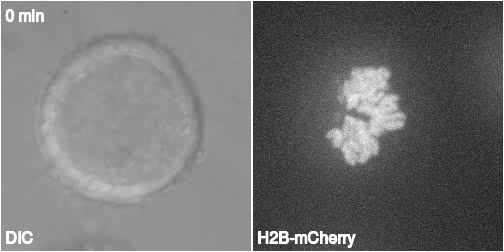
\includegraphics[scale=.3]{testvideo.png}}]{}{}%
        {testvideo.avi}
    \end{center}
  \end{block}
\end{frame}

\end{document}
